%!TEX TS-program = lualatex
%!TEX encoding = UTF-8 Unicode
%% (this document must be compiled with LuaLaTeX) 
%% PFPE matlab gravity tie gui docs
%% 
%% Formatting loosely based on the Overleaf Software Manual and Technical Document Template	
%% 									

\documentclass{pfpe-manual}

% Packages used in this example
\usepackage{graphicx}  % for including images
\usepackage{microtype} % for typographical enhancements
\usepackage[letterpaper,top=4.2cm,bottom=4.2cm,left=3.5cm,right=3.5cm]{geometry} % for setting page size and margins

% Custom macros
\newcommand{\doclink}[2]{\href{#1}{#2}\footnote{\url{#1}}}
%\newcommand{\cs}[1]{\texttt{\textbackslash #1}}

% Frontmatter data; appears on title page
\title{gravity tie gui manual - MATLAB}
\version{1.0.0}
\author{Masako Tominaga, Jasmine Zhu, James Kinsey, Stefano Suamn, Hannah F. Mark, PFPE staff}
\license{CC-BY 4.0}
%%%%%%%%%%%%%%%%%\softwarelogo{\includegraphics[width=8cm]{figs/grav_photo}}

\begin{document}

\maketitle

\tableofcontents
\newpage

\section{Introduction}

This MATLAB-based GUI is designed to record the tie process for a DgS gravimeter installed on a vessel, compute the bias of the meter, and then generate a report that contains all the calibration algorithms. The GUI can perform the calculation for a standard tie or for a land tie.

\section{How to start the GUI}
\label{start}

First, download the files for the program from \url{https://github.com/PFPE/gravtiegui_MATLAB}. If you download the files as a zip archive, unpack the contents of the archive into a folder where you will run the program.

Open MATLAB, and navigate to the folder where the gravity tie GUI files live. This should include \texttt{GravityTie.m} and \texttt{GravityTie.fig}, as well as a folder named \texttt{database/} and some other \texttt{.m} files. In the MATLAB file browser (left panel of the standard window), right-click on the \texttt{database/} folder and select ``Add to Path > Selected Folders and Subfolders''.

In the MATLAB command prompt, run \texttt{GravityTie} to start the GUI.

\begin{figure}[ht!]
\centering
\includegraphics[width=\textwidth]{figs/GUI_window.png}
\caption{The GUI window, before any data has been entered.}
\label{guiwindow}
\end{figure}


\begin{figure}[ht!]
\centering
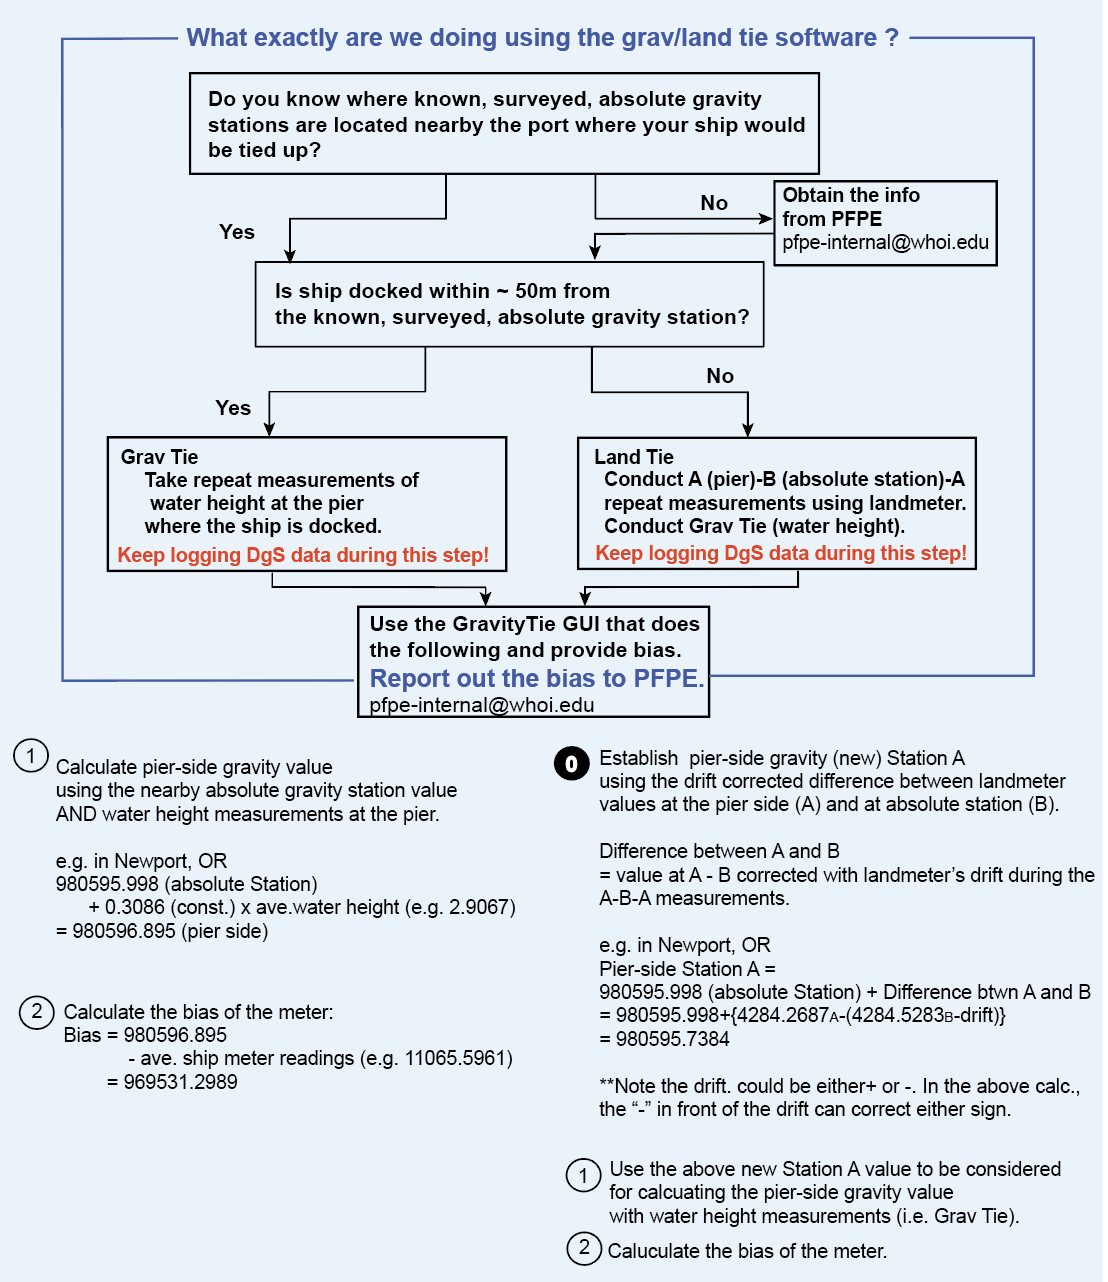
\includegraphics[width=\textwidth]{figs/flowchart.png}
\caption{Overall flow of the tie process, and a brief overview of the calculation performed.}
\label{flowchart}
\end{figure}

\section{Gravity tie terminology}
\begin{itemize}
\item \textbf{Absolute gravity (base) station:} surveyed station with an absolute gravity value. These are typically located near major ports or piers, but may also be found in obscure places such as public buildings, parks, airports, and roadside areas. PFPE has access to an up-to-date national and international proprietary database through connections with the National Geospatial Agency. In this manual, this absolute or base station is termed “Station B” while where the ship is tied up at the dock is termed as “Station A”. 

\item \textbf{Bias (of the gravimeter):} a meter-specific gravity reading baseline determined against a known absolute gravity value from a base station. This is the value that needs to be historically tracked to monitor drift. 

\item \textbf{Drift (of the gravimeter):} drift of gravimeter reading baseline, typically a linear regression over time. Calculating drift requires at least two ties (ideally at the beginning and the end of a cruise).  

\item \textbf{Water height measurement (m):} the dock to the sea-level distance at a given spot at the pier adjacent to the ship. This measurement is taken 3 times at 30 minute intervals for a gravity tie.

\item \textbf{Gravity tie:} process to measure gravimeter bias using an absolute base station (station B) that can be found within \textasciitilde50 m from where the vessel is docked. The bias is calculated by comparing to the known gravity value at the base station with repeat water height measurements.

\item \textbf{Land tie:} process to establish an ad-hoc gravity base station at the pier (Station A) when known base stations are >> 50m from where the vessel is docked. In this case, the gravity value at Station B (base station) is unable to represent the gravity at the dock, so we must introduce a new gravity station (Station A) at the pier where ship is docked. Then a measurement is made at the known gravity station (Station B), and finally back at Station A with repeat measurements using a land meter.  This is known as an A-B-A tie. The land tie is completed by conducting a gravity tie with water height measurements at the pier (so when we say “Land Tie”, that inevitably includes a regular gravity tie as the last step of the process – see the flow chart in Fig \ref{flowchart}). The bias of the meter will then be determined by comparing to the calculated gravity value at Station A, which was in turn calculated by referencing to Station B.

\end{itemize}


\section{Step-by-step instructions}
\label{tie-instructions}

\begin{figure}[ht!]
\centering
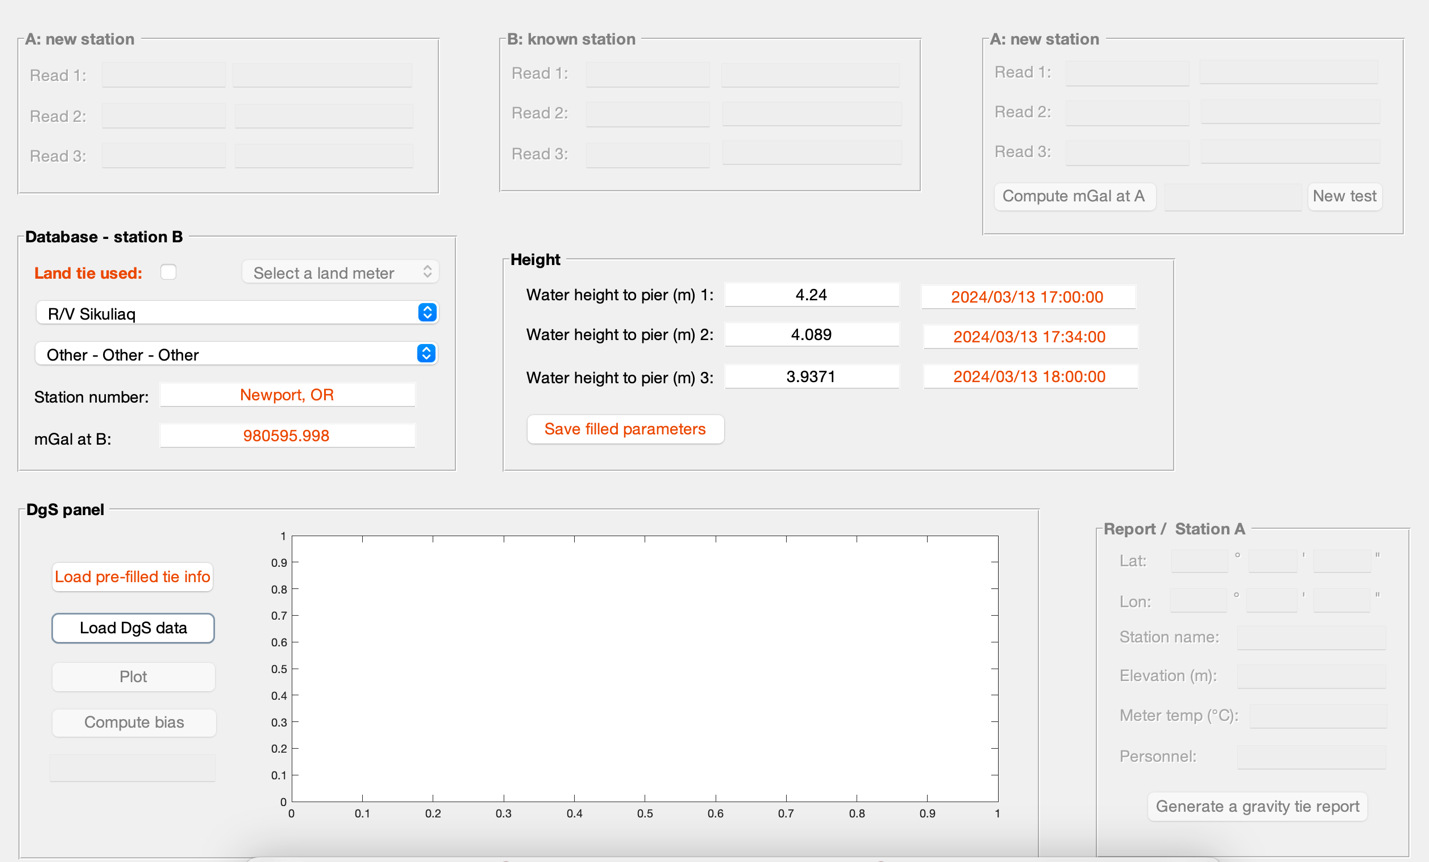
\includegraphics[width=\textwidth]{figs/window_with_heights.png}
\caption{The GUI window, with metadata and water heights entered.}
\label{gui:heights}
\end{figure}

\begin{figure}[ht!]
\centering
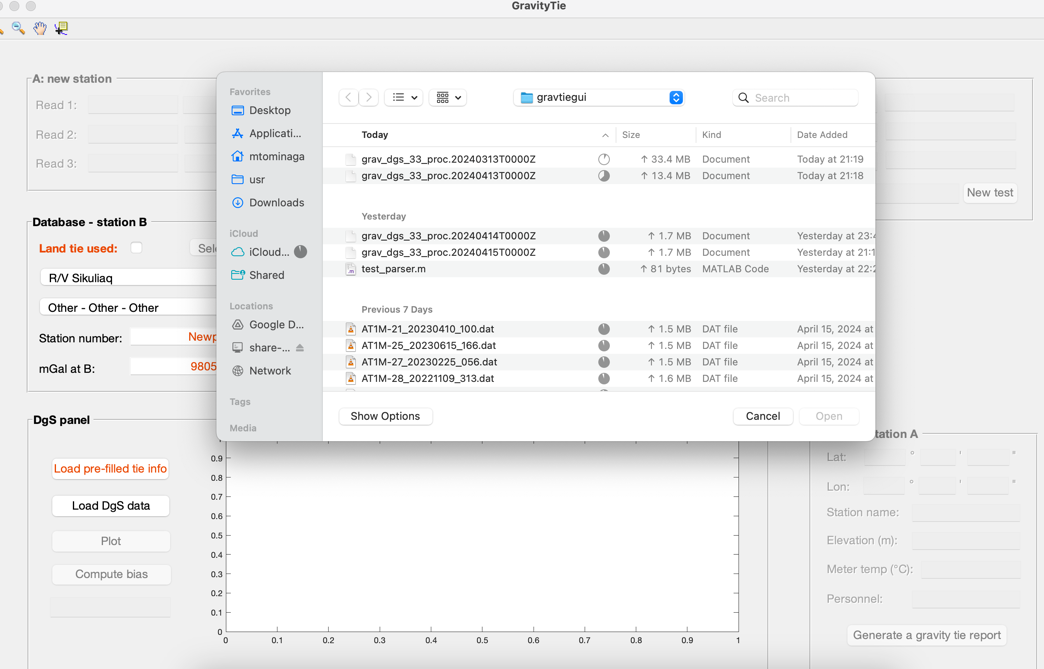
\includegraphics[width=\textwidth]{figs/select_dgs.png}
\caption{Selecting DGS files to load data.}
\label{gui:select}
\end{figure}

\begin{figure}[ht!]
\centering
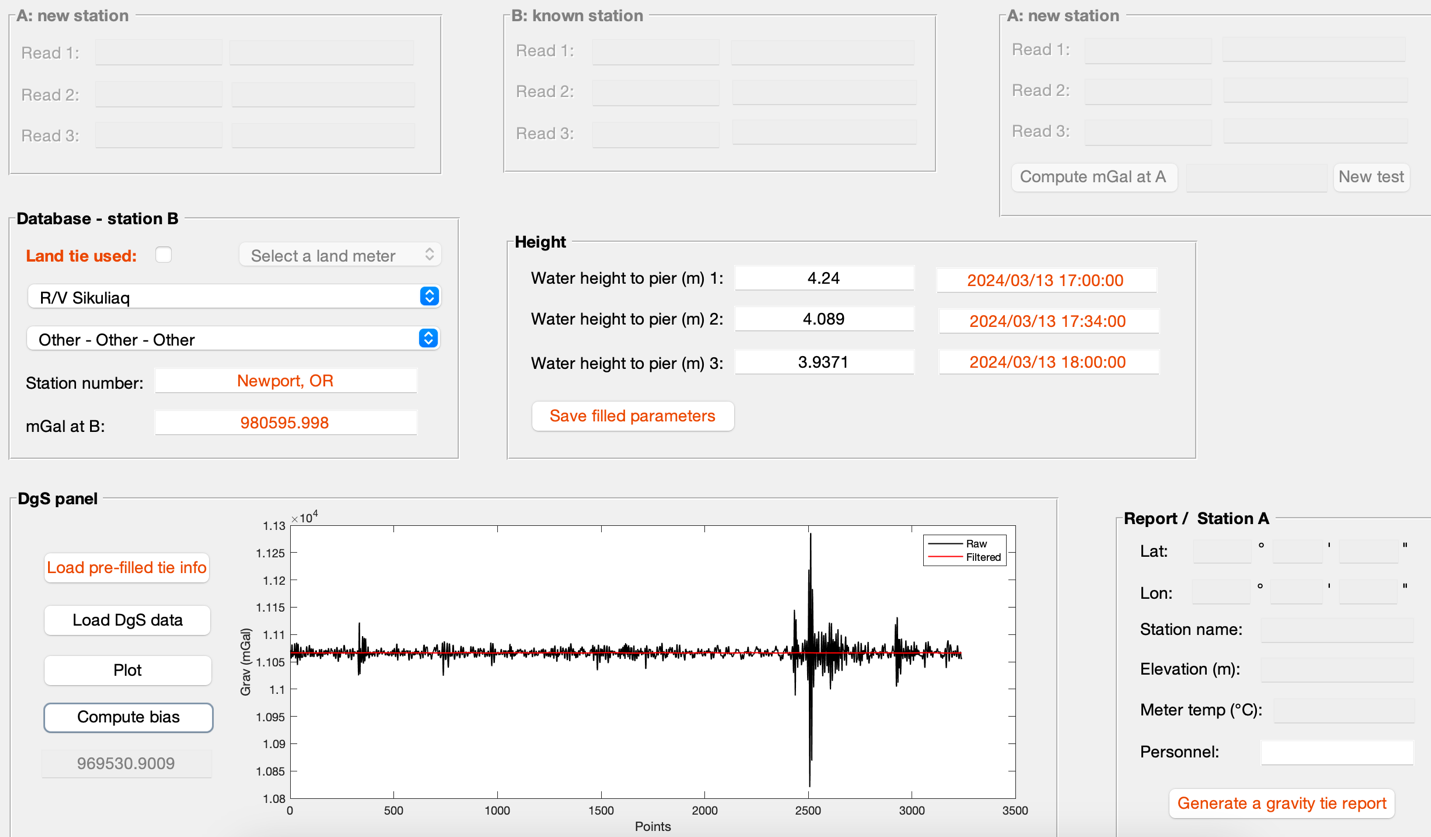
\includegraphics[width=\textwidth]{figs/plot_dgs.png}
\caption{After loading DGS data, it can be plotted (with and without gaussian filter applied).}
\label{gui:plot}
\end{figure}

\begin{figure}[ht!]
\centering
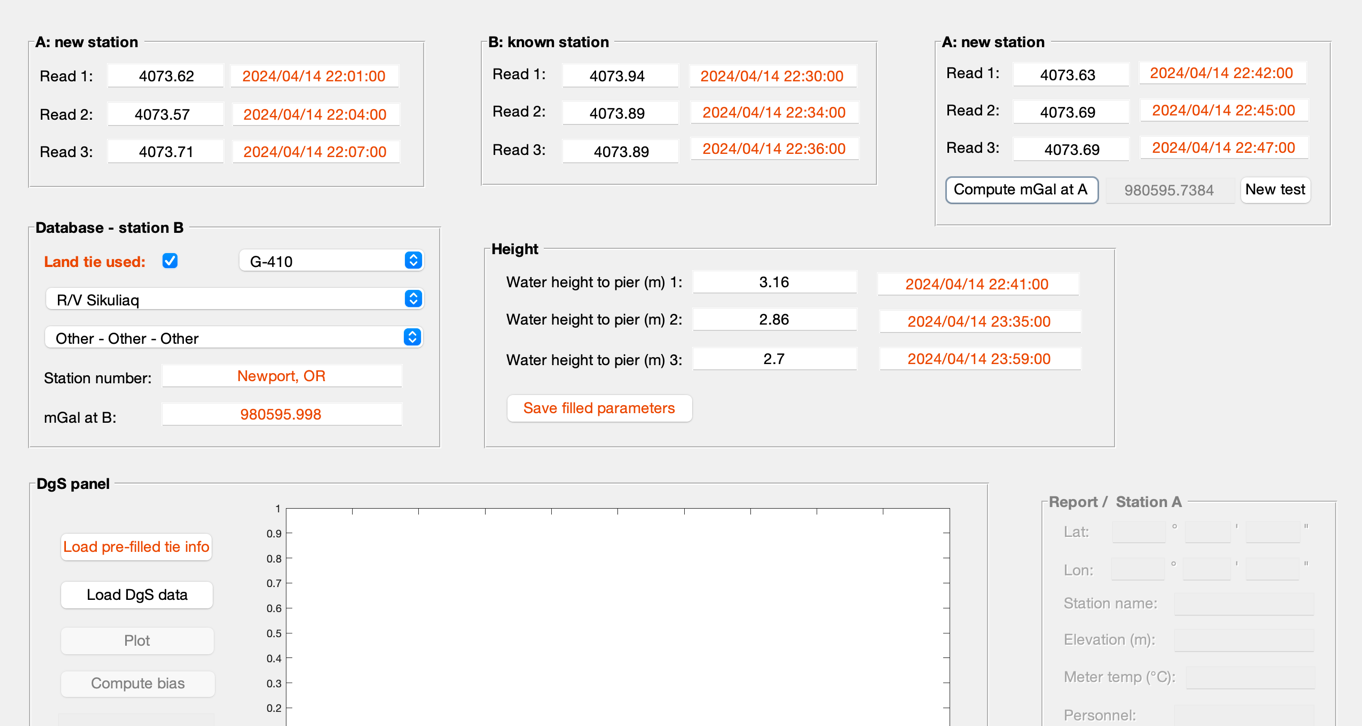
\includegraphics[width=\textwidth]{figs/land_tie_filled.png}
\caption{The GUI window with all of the land tie measurements entered.}
\label{gui:landtie}
\end{figure}

\begin{figure}[ht!]
\centering
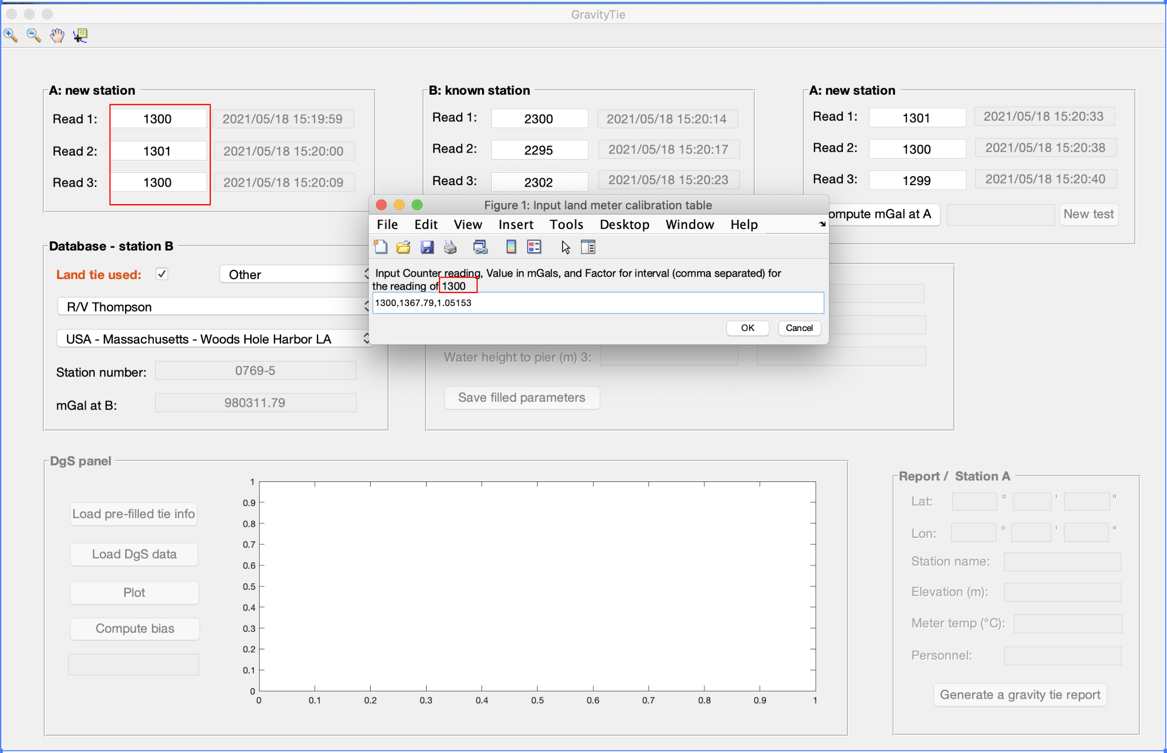
\includegraphics[width=\textwidth]{figs/land_tie_cal.png}
\caption{If a land meter calibration file is not in the database, the user will have to enter calibration information to complete the land tie.}
\label{gui:cal}
\end{figure}




\begin{enumerate}
\item Start the GUI (see Section~\ref{start})
\item Enter the tie metadata
    \begin{itemize}
    \item Select a ship from the dropdown menu.
    \item Select a station from the dropdown menu. This will populate the fields below the menu with the station ID and absolute gravity value for that station. If you choose `Other', you will need to enter a station name or ID, and an absolute gravity value.
    \end{itemize}
\item Make pier water height measurements
    \begin{itemize}
    \item Measure water height at the pier 3 times, with \textasciitilde 30 minutes elapsing between measurements (Fig \ref{gui:heights}). Enter each water height (in meters) in the appropriate field in the GUI. When you click out of the field after a value is entered, the current time will automatically be entered in the adjacent field.
    \item\textbf{Optional, recommended:} use the ``Save filled parameters'' button to save your progress in a .mat file. This file can be reloaded into the GUI later if you need to close and re-open the window (see Section~\ref{save-re}).
    \item[\textbf{Note:}] If you aren't entering the water height measurements at the time they are taken, you can manually adjust the timestamps. The times you enter \textbf{must be in UTC} and must \textbf{exactly follow the formatting} of the automatically generated timestamps.
    \end{itemize}
\item Load the DGS gravimeter data covering the time period of the water height measurements (Fig \ref{gui:select}). The data should be the output files from the ``FILE DATA'' serial from the AT1M front panel, or output from the DGS laptop. If you don't know which files to use, contact PFPE and attach example(s) of available data files (pfpe-internal@whoi.edu).
\item Plot the data (Fig \ref{gui:plot}). Data outside of the time window of the water height measurements will not be shown. A Gaussian filter will be applied before the data is plotted.

\item \textbf{For land ties only:}
    \begin{itemize}
    \item Check the ``Land tie'' check box, and select a land meter from the dropdown list. 
    \item Fill out the three sets of land meter readings made at station A (pier side), B (base station, and A again (Fig \ref{gui:landtie}). Gravity is measured 3 times at each station. Remember to clamp, move, and relevel the meter between each of these three measurements to ensure independent measurements. Input times (UTC) of the readings will be automatically recorded as with the water heights, but can be manually adjusted as needed.
    \item Click ``Compute mGal at A'' to compute the reference value at Station A which will be used for the bias calculation. This button will also trigger the calibration of the land meter readings based on the calibration table for the meter selected previously. \textbf{Note:} if the selected meter is ``Other,'' the user will be asked to manually type in the information for calibration, which consists of sets of counter readings, values in mGals, and factors for each counter interval in comma-separated lists (Fig \ref{gui:cal}).
    \end{itemize}

\item Compute bias
\item Fill in your name as ``Personnel'' who collected the tie. If taking a land tie, also fill in the other fields in the ``report'' panel: the location of the ship (station A), elevation, land meter temperature.
\item Click the ``Generate a gravity tie report'' button in the lower right corner of the window. This will write a .txt file (Figs \ref{rep:tie} and \ref{rep:landtie}). Send this file to PFPE and include it with data files sent to R2R.
\end{enumerate}

\begin{figure}[ht!]
\centering
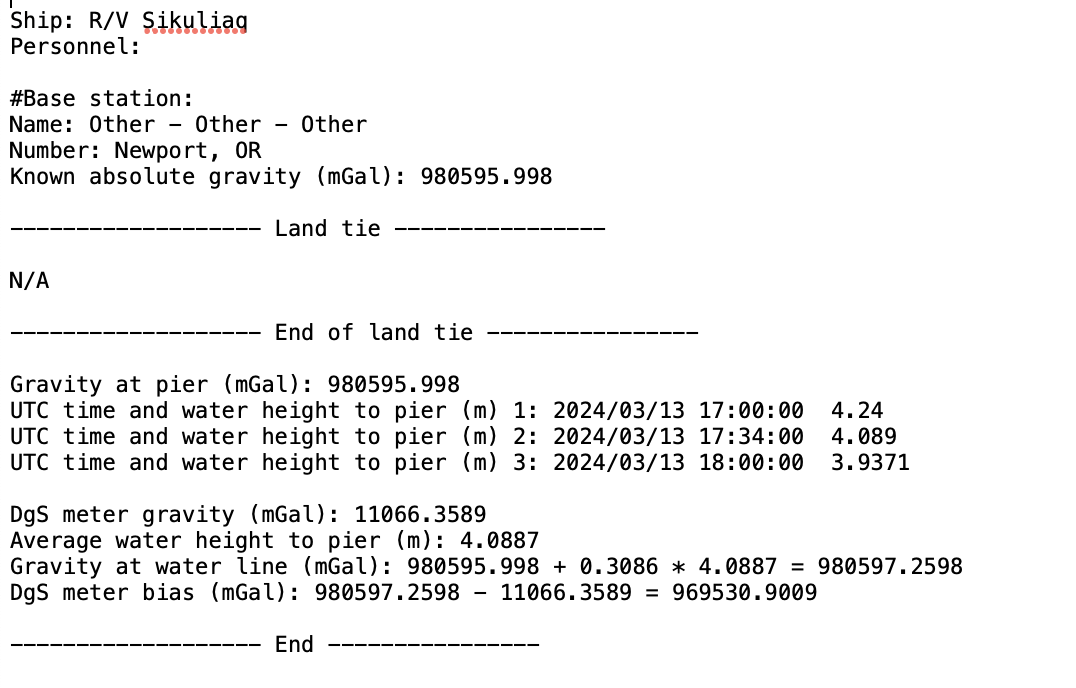
\includegraphics[width=\textwidth]{figs/tie_report.png}
\caption{An output .txt file from a gravity tie.}
\label{rep:tie}
\end{figure}

\begin{figure}[ht!]
\centering
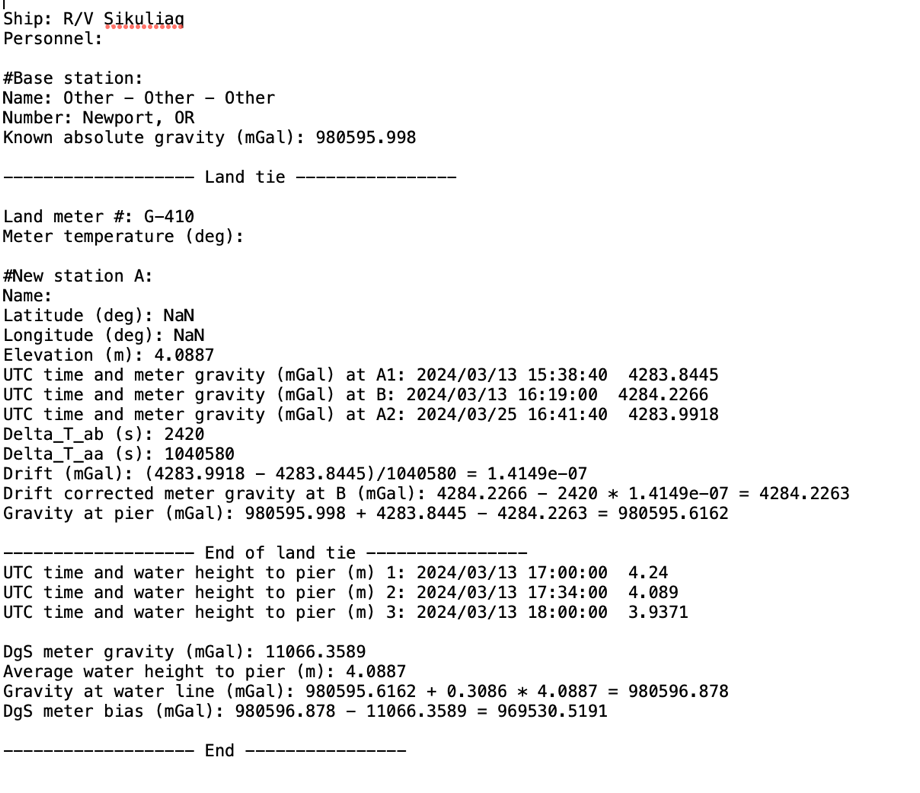
\includegraphics[width=\textwidth]{figs/land_tie_report.png}
\caption{An output .txt file that includes a land tie.}
\label{rep:landtie}
\end{figure}




\subsection{Saving and re-reading tie information}
\label{save-re}
The ``Save filled parameters'' button will write the information entered in the GUI thus far to a .mat file. If you need to close and restart the GUI, saved parameters can be re-read later using the ``Load pre-filled tie info'' button. Note that re-loaded parameters may not be editable in the GUI (this is a known bug) but you can also open the saved .mat file in MATLAB (independent of the GUI), edit the data contained in the ``tie'' struct, re-save, and then re-load it if needed.


\subsection{Database files}
\label{datab}

This program ships with a set of database files that contain some information on ships, stations, and land meter calibrations. The files are used to populate the dropdown menus in the GUI interface, and are also used to fill in known values for things like base station gravity and land meter calibration tables where possible. Note that it is possible to select ``Other'' for your station, ship, and/or land meter if the appropriate options are not on the lists provided. However, in that case, you may need to manually enter quantities such as station gravity and/or land tie calibration information, and the program may not be able to read your gravimeter data files as the file format is ship-dependent.

To propose updates or additions to the database files, please contact PFPE at pfpe-internal@whoi.edu.

\section{Why do we take gravity ties?}
Any marine gravimeter onboard your vessel is a so-called “relative” gravimeter. This means we do not have scientifically meaningful gravity values until some corrections are made. One of of these corrections is the \emph{drift} of the gravimeter. This is a timeseries with a linear regression character shown by the data due to the nature of any relative gravimeter, where the response of internal mechanical components may have changed due to platform vibration, and or expected wear/tear/aging of the materials, etc. To obtain the drift (and to document historical drift rates of the meter), we need to know the value that your gravimeter is reading with respect to an absolute (or “reference”) value. This is provided by a nearby gravity station at the beginning and end of the timeseries, typically for each research cruise. This is why PFPE often asks: “please do the tie”; “have you done tie?”; “when did you do the tie last time” etc. 

\textbf{The underway gravity data sent to R2R can only be scientifically useful if the tie information accompanies and is archived with the data.}

If the operator cannot determine if they should do a tie, please reach out to pfpe-internal@whoi.edu for advice and guidance.

\section{Help!}
\label{helphelp}

\subsection{Troubleshooting}

\subsubsection{MATLAB can't read my DGS data files}
First, make sure that you are using the `laptop' data files rather than the raw files, as those are what this program is designed to read. If that still doesn't work, contact PFPE with a sample of the unreadable file. It may be that the program doesn't yet know how to read files from your ship, as there are variations in gravimeter file format between vessels/instruments. Note that you can take and save all of the measurements necessary for a gravity tie in a .mat file and wait until later to compute the bias if there are issues with reading gravimeter files.

\subsubsection{The calculated bias number is really weird}
There are several possibilities here, but they all boil down to: there's probably some miscommunication between us and the program. Maybe the timestamps for measurements are incorrect, or the DGS file is not being read properly, or there is some mixup with measurement units. Double-check all of the data that you have input: remember that water height measurements should all be in meters, and timestamps must be UTC rather than local time to match what is recorded in the gravimeter files.

\subsubsection{I have some other question that's not answered here}
For specific assistance, contact PFPE at \href{mailto:pfpe-internal@whoi.edu}{pfpe-internal@whoi.edu}.

\section{Appendix: BGM3 ties}
These instructions are from previous user manuals for BGM3 meters and their associated GUI program. The descriptions of the GUI and its buttons and windows do not match this MATLAB-based GUI for DGS meters.

\subsection{Ship-to-shore, no land tie}
A gravity tie is executed to determine the bias (offset), in mGal, of the gravimeter, allowing the user to relate the sensor’s relative gravity measurement to a known and accurate benchmark site which is considered stable and has been surveyed in by a very precise land based gravimeter. As such, doing a gravity tie requires the gravity value of an established gravity station where the ship is docked. The software includes a database of known, trusted gravity stations that will be expanded over time. If the ship’s docking location does not have a station in the database, contact pfpe-internal@whoi.edu for a search in an extended database. If no gravity station exists at the ship’s exact docking location, a land tie is required before executing the gravity tie, to determine the gravity value of “station A” at the ship pier. 

A gravity tie takes about one hour of time, but it is mostly automated in the software. Instructions to use the gravity tie interface are:
\begin{itemize}
\item If the software detects a system malfunction or a “data not valid” flag during the gravity tie, the gravity tie will automatically abort and the abort reason will be displayed on the gravity tie window. In this case, the system malfunction or “data not valid” should be investigated before restarting the gravity tie again
\end{itemize}

\subsection{Land tie instructions}
A land tie is executed (and necessary) if no established gravity stations are available immediately next to (i.e., within 50m) where the ship is docked. The purpose of a land tie is to determine the gravity value (in mGal) at the location where the ship is docked (station A – new station), using: a) information from a land gravity meter and b) the gravity value of a known and well established gravity station (station B – known station).

When a land tie is required, a technician should use a land meter to record:
\begin{enumerate}
\item The time (and reading from the land gravimeter) at station A (repeated three times)
\item The time (and reading from the land gravimeter) at station B (repeated three times)
\item The time (and reading from the land gravimeter) at station A again (repeated three times)
\end{enumerate}
When this data has been collected, the “Land Tie” button on the GUI opens a window to determine the value of the gravity at the pier (station A). Instructions to use the land tie interface are:
\begin{enumerate}
\item Click the “Land tie” button on the GUI to open the land tie interface
\item Click “NEW” to start a new land tie
\item Enter the first set of three land meter readings and times for station A in the first station A block
\item Enter the set of three land meter readings and times for station B in the station B block
\item Enter the second set of three land meter readings and times for station A in the second station A block
\item In the “Database – section B” block, select the appropriate ship, and the gravity station used for station B from the database. If the station B you used is not in the database, select “Other – Other – Other” and enter all the information required to fill out this block, including the “mGal at pier” field. NOTE: this “mGal at pier” field is NOT the value of the gravity at the pier where the ship is docked, but the value of the gravity of station B (known station)
\item In the “New Station – station A” section, enter the latitude and longitude of the new station (A) that you are establishing (i.e., from a handheld GPS receiver), assign a name to the new station and use the text box below to enter any note that can help in better identify the location of the station (for example, indicate distances from bollards, from pier ends, from easily recognizable landmarks, etc…). These notes are useful to locate again the new station in the future
\item In the “Additional information” section, enter the name(s) of the personnel who used the land meter for this land tie and/or filled out the information in the land tie window. Enter the land meter temperature recorded during the readings in the field, and select the serial number of the land meter used. The software automatically uses the appropriate calibration table for the particular land meter S/N to compute the reading-to-mGal conversion
\item Click “COMPUTE” to compute the value of the gravity at station A. The computed value will be displayed to the right of the “COMPUTE” button
\item If the value computed is acceptable, click the “ACCEPT” button to generate and save a report
\end{enumerate}


\end{document}
